\documentclass[10pt, twoside, openany]{book}

\usepackage[a4paper, top=2.5cm, bottom=2.5cm, left=3cm, right=3cm]{geometry}
\usepackage[utf8]{inputenc}
\usepackage[italian]{babel}
\usepackage{cite}
\usepackage{graphicx}
\usepackage{fancyhdr}
\usepackage[Lenny]{fncychap}
\usepackage{frontespizio}

\pagestyle{fancy}
\fancyhead{}
\fancyhead[LE]{\rightmark\hfill\leftmark}
\fancyhead[RO]{\leftmark\hfill\rightmark}
\bibliographystyle{plain}

\begin{document}
\begin{frontespizio}
\Universita{Roma Tor Vergata}
\Dipartimento{Ingegneria Civile e Ingegneria dell'Informazione}
\Corso{Ingegneria Informatica}
\Annoaccademico{2023/2024}
\Titolo{Titolo della tesi}
\Candidato[0316179]{Matteo Fanfarillo}
\Relatore{Giuseppe Bianchi}
\Correlatore{Francesco Gringoli}
\Logo{logo.png}
\end{frontespizio}

\begin{flushright}
\null\vspace{\stretch{1}}
\textit{[Citazione]}
\vspace{\stretch{2}}\null
\end{flushright}

\tableofcontents
\listoffigures
\listoftables

\chapter{Introduzione}
[TODO]

\chapter{Interfacce e funzionamento della eSIM}
[TODO]

%\cite{Android-docs}
%\cite{GSMA}

\chapter{Analisi della sicurezza della eSIM a run-time}
[TODO]

\chapter{Analisi della sicurezza della eSIM a boot-time}
\section{Funzionamento del boot della eSIM}
[TODO]

\section{Potenziali vulnerabilità}
[TODO]

\section{Prove sperimentali}
[TODO]

\chapter{Conclusione}
[TODO]

\bibliography{Bibliography}

\chapter*{Ringraziamenti}
[TODO]

%\begin{figure}
%  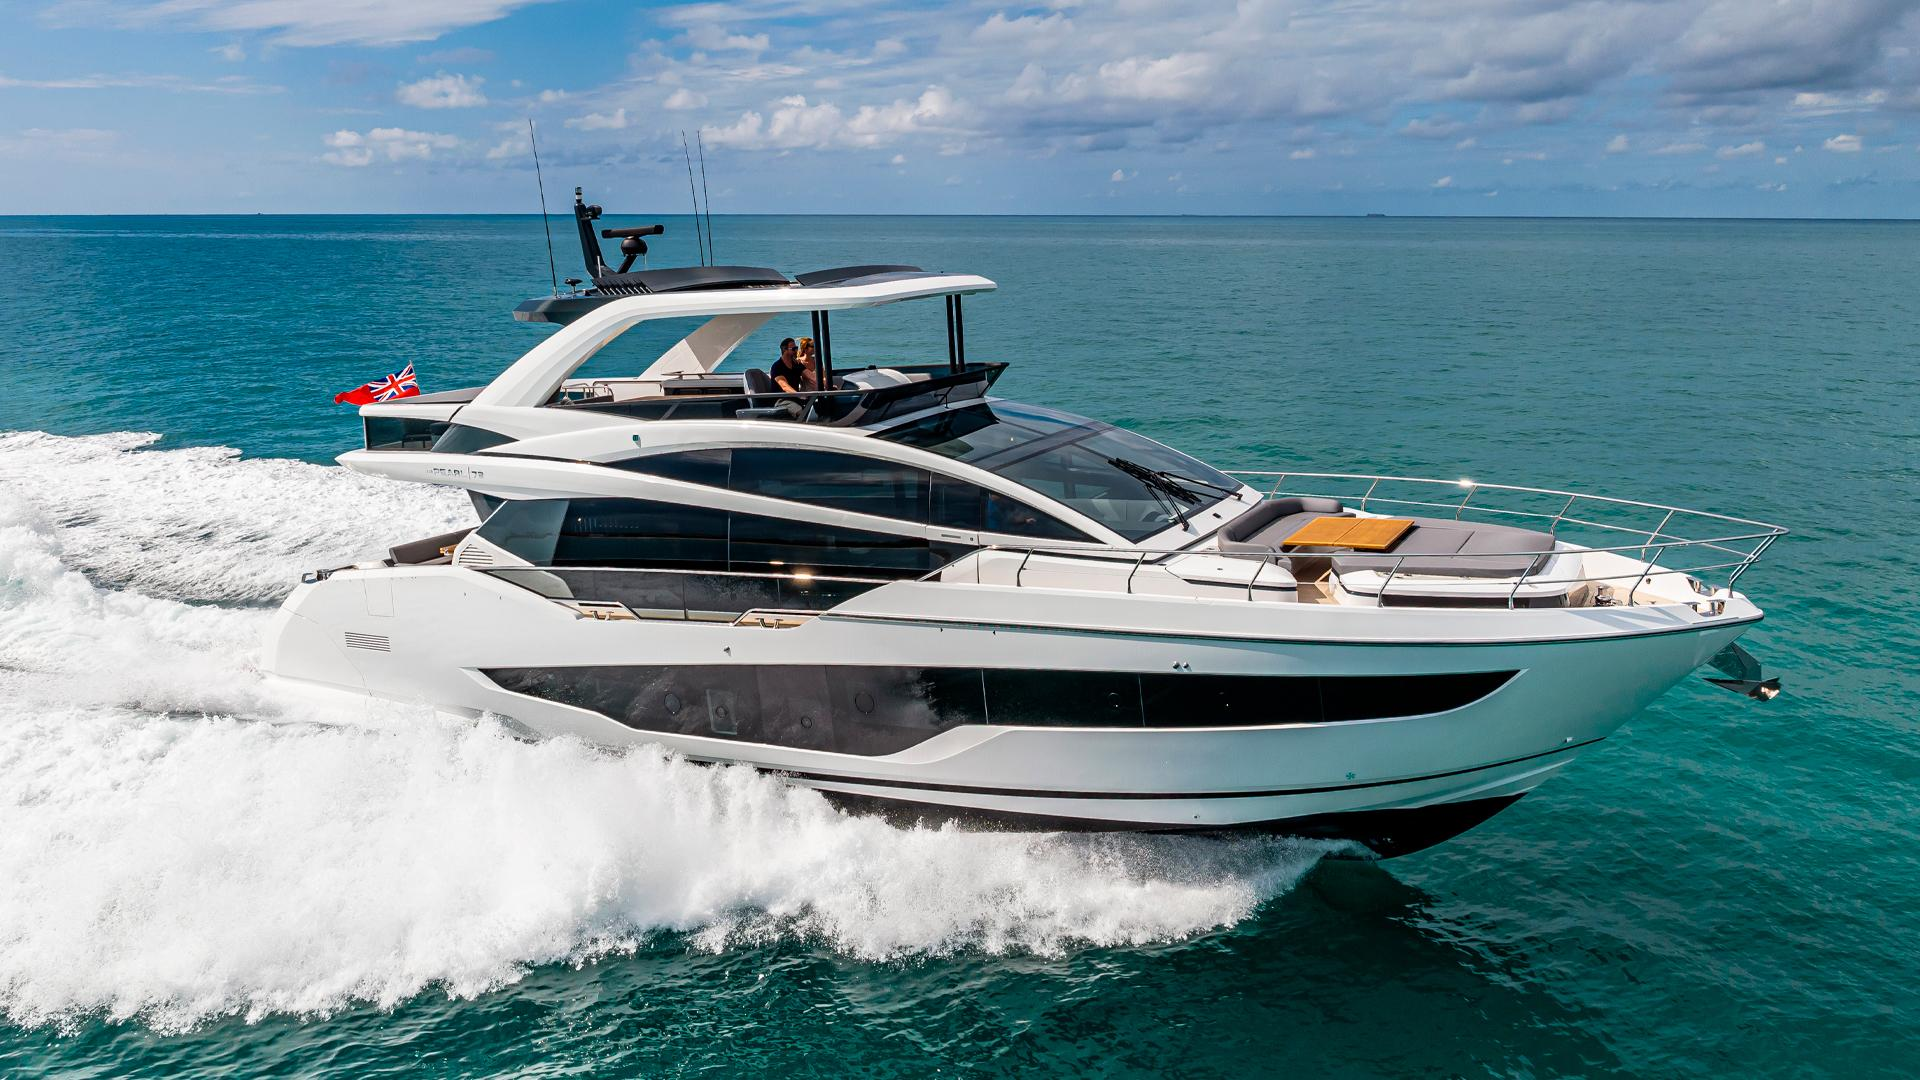
\includegraphics[width=\linewidth]{boat.jpeg}
%  \caption{A boat.}
%  \label{fig:boat1}
%\end{figure}
%Figure \ref{fig:boat1} shows a boat.

%\section{Sezione}
%This is where you tell people why they should bother reading your article.

%\subsection{Sottosezione}
%Hi.

%\begin{table}[h!]
%  \begin{center}
%    \caption{Your first table.}
%    \label{tab:table1}
%    \begin{tabular}{l|c|r} % <-- Alignments: 1st column left, 2nd middle and 3rd right, with vertical lines in between
%      \textbf{Value 1} & \textbf{Value 2} & \textbf{Value 3}\\
%      $\alpha$ & $\beta$ & $\gamma$ \\
%      \hline
%      1 & 1110.1 & a\\
%      2 & 10.1 & b\\
%      3 & 23.113231 & c\\
%    \end{tabular}
%  \end{center}
%\end{table}

\end{document}